\section{Project 1 - Histogram Equalization}

\subsection{Project Proposal}
In this project we implement histogram equalization. First, plot the histogram of an image, then implement histogram equalization and display the equalized image and histogram. Test images are \emph{Fig1.jpg, Fig2.jpg}.

\subsection{Preliminaries}
Let $r$ denote the intensity of a pixel in the original image and $r \in [0,L-1]$. We consider a transformation \begin{equation}s=T(r) ~~~~ 0 \leq r \leq L-1 \end{equation} that produce an output intensity level $s$ for every pixel in the input image having intensity $r$. We assume that:
\\ \textbf{(a)} $T(r)$ is a monotonically increasing function in the interval $0 \leq r \leq L-1$; and \\
\textbf{(b)} $0 \leq T(r) \leq L-1$ for $r \in [0, L-1]$. \\
Condition \textbf{(a)} and \textbf{(b)} guarantee the existing of inverse function $r=T^{-1}(s)$ which is monotonically increasing. 
The central idea is that \emph{intensity levels of an image can be viewed as random variables in the interval $[0, L-1]$ and can be described by probability density function (PDF).} Let $p_r(r)$ and $p_s(s)$ to be the PDF of $r$ and $s$ respectively. Thus we can apply the basic result of probability theory that \emph{if $T(r)$ is differentiable over the range of interest, we have this below relationship between $p_r(r)$ and $p_s(s)$: }
\begin{equation} p_s(s)=p_r(r) \left| \frac{dr}{ds} \right| \label{equ:basicprob} \end{equation}
Then consider the cumulative distribution function(CDF) which is exactly used here as the transformation function $T(r)$ \begin{equation} s=T(r)=(L-1) \int_0^r p_r(w)dw  \label{equ:histEquTrans} \end{equation}
Now we are ready to prove the transformation really does the histogram equalization. Firstly, compute the derivatives. The last $=$ is from the assumption \textbf{(a)} stating the monotonically increasing.
\begin{equation} \frac{ds}{dr}=\frac{dT(r)}{dr}=(L-1)p_r(r) = \left| \frac{ds}{dr} \right| \end{equation}
Thus, substituting the result for Eq.\ref{equ:basicprob}, we get the desired result
\begin{equation} p_s(s) = p_r(r) \frac{1}{(L-1)p_r(r)} = \frac{1}{L-1} \end{equation}
which show $p_s(s)$ follows uniform distribution.

\subsection{Histogram equalization}
Histogram equalization on an image of size $M\times N$ is like a discrete version of the process in the preliminaries section. \begin{equation} p_r(r_k)=\frac{n_k}{MN} ~~~~~~ k=0,1,2,...,L-1  \end{equation} where $n_k$ is the number of pixels that have intensity $r_k$. The discrete form of Eq.\ref{equ:histEquTrans} is \begin{equation} s_k=T(r_k)=(L-1)\sum_{j=0}^k p_r(r_j)=\frac{L-1}{MN} \sum_{j=0}^k n_k ~~~~~~ k=0,1,2,...,L-1 \end{equation}
Based on these discrete form equation, I implement the matlab function and test them on \emph{Fig1.jpg, Fig2.jpg} and get the results listed in \ref{fig:result1} and \ref{fig:result2} respectively.
\begin{figure}[h!]
	\centering
	\begin{subfigure}[b]{0.45\linewidth}
		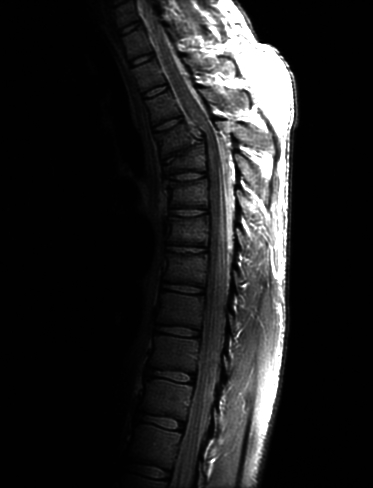
\includegraphics[width=\linewidth]{myfigure/p1/Fig1.jpg}
		\caption{}
		\label{fig:Fig1}
	\end{subfigure}
  	\begin{subfigure}[b]{0.45\linewidth}
		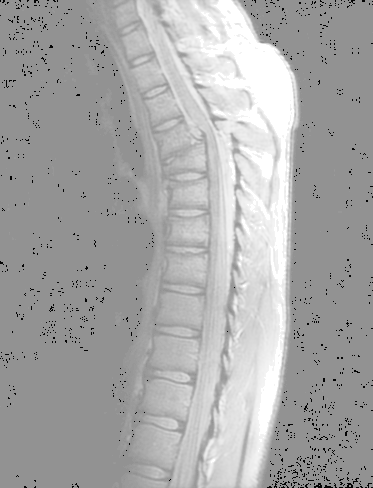
\includegraphics[width=\linewidth]{myfigure/p1/g1.png}
		\caption{}
		\label{fig:g1}
	\end{subfigure}
	\begin{subfigure}[b]{0.45\linewidth}
    	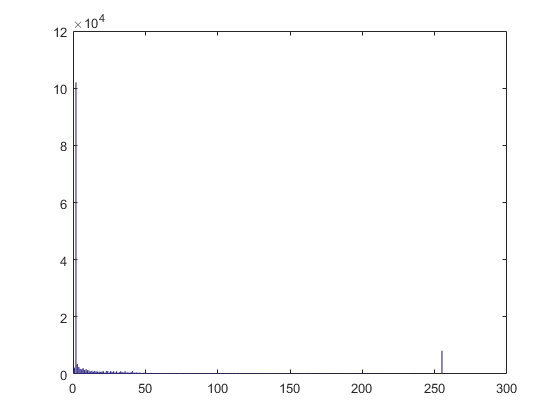
\includegraphics[width=\linewidth]{myfigure/p1/fbar1.png}
    	\caption{}
    	\label{fig:fbar1}
  	\end{subfigure}
	\begin{subfigure}[b]{0.45\linewidth}
    	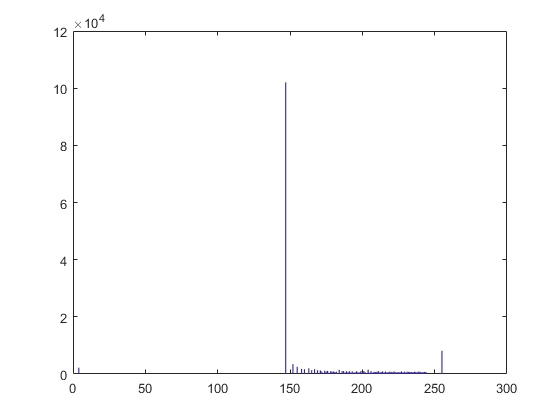
\includegraphics[width=\linewidth]{myfigure/p1/gbar1.png}
    	\caption{}
    	\label{fig:gbar1}
  	\end{subfigure}
  	\caption{Results of Fig1.jpg. (a)Original image. (b)Processed image after applying histogram equalization. (c)Histogram of original image. (d)Histogram of processed image.}
  	\label{fig:result1}
\end{figure}

\begin{figure}[h!]
	\centering
	\begin{subfigure}[b]{0.45\linewidth}
		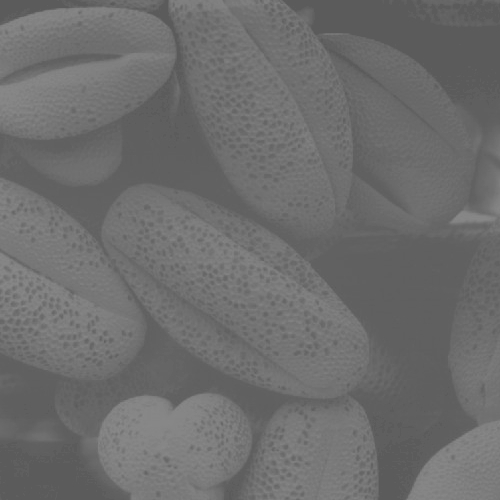
\includegraphics[width=\linewidth]{myfigure/p1/Fig2.jpg}
		\caption{}
		\label{fig:Fig2}
	\end{subfigure}
	\begin{subfigure}[b]{0.45\linewidth}
		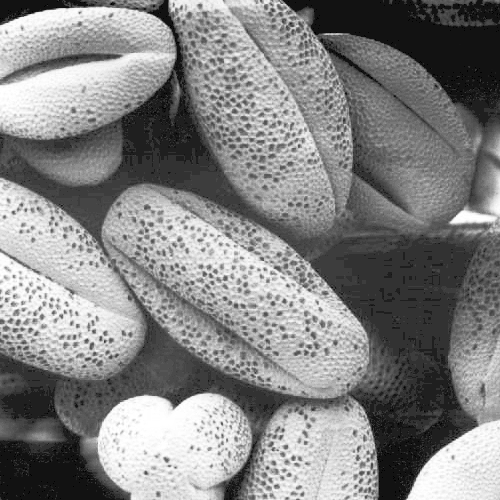
\includegraphics[width=\linewidth]{myfigure/p1/g2.png}
		\caption{}
		\label{fig:g2}
	\end{subfigure}
	\begin{subfigure}[b]{0.45\linewidth}
    	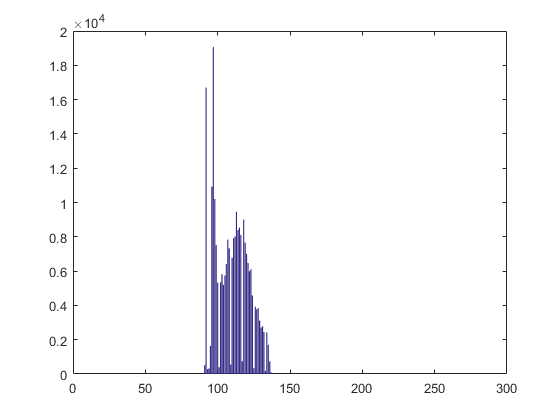
\includegraphics[width=\linewidth]{myfigure/p1/fbar2.png}
    	\caption{}
    	\label{fig:fbar2}
  	\end{subfigure}
	\begin{subfigure}[b]{0.45\linewidth}
    	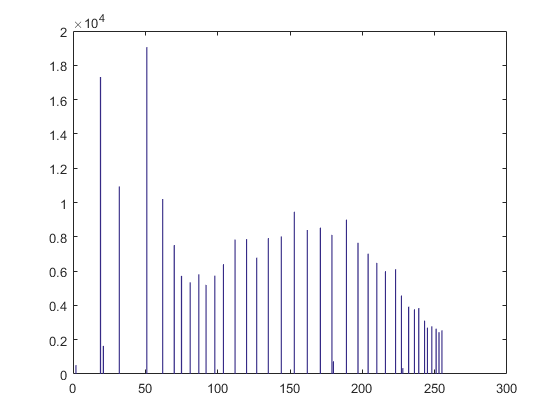
\includegraphics[width=\linewidth]{myfigure/p1/gbar2.png}
    	\caption{}
    	\label{fig:gbar2}
  	\end{subfigure}
  	\caption{Results of Fig2.jpg. (a)Original image. (b)Processed image after applying histogram equalization. (c)Histogram of original image. (d)Histogram of processed image.}
  	\label{fig:result2}
\end{figure}

\clearpage

\subsection{Discussion}
We can see that histograms are quite different from continuous functions because there are gaps between each horizontal value. So the histogram of the equalized image is like a sparse version of the original image. The result of Fig2(low contrast ratio) shows an increasing on contrast ratio and it's more useful than the original result. However, Fig1(high contrast ratio) is not a good example of histogram equalization. The affect is just like a intensity transition. We can simply draw a not so serious conclusion that histogram equalization is useful for images with low contrast ratio but not for images with high contrast ratio.

\subsection{Implementation}
There is some key part of my implementation.
\lstset{language=Matlab}
\begin{lstlisting}
function [x, y] = histShow( imgf )
%HISTSHOW display the histogram graph of the imgf
% x - the horizontal axis of histogram, 
% y - the vertical axis of histogram
g = imgf(:) + 1;
n = length(g);
x = (1 : 256);
y = zeros(1, 256);
for i = (1 : n)
    y(g(i)) = y(g(i)) + 1;
end

end

function [ imgg ] = histEqual( imgf )
%HISTEQUAL 
%   
[x, y] = histShow(imgf);
T = zeros(1, 256);
a = 0;
g = imgf(:);
n = length(g);
for i = (1 : 256)
    T(i) = a + y(i);
    a = T(i);
end
T = round(255 * T / n);
for i = (1 : n)
    g(i) = T(g(i)+1);
end
imgg = reshape(g, size(imgf));

end
\end{lstlisting}




